%%%%%%%%%%%%%%%%%%%%%%%%%%% COORDINATESYSTEMS
% COORDSYS (ORIGOCOORDINATENAME, WIDTH, HEIGHT)
% Draws a Coordinatesystem around ORIGOCOORDINATENAME with a width of WIDTH and a height of HEIGHT, 
% names the beginning and end of axes, southwest corner, northwest corner, 
\newcommand{\CoordSys}[3]{
\coordinate (XY#1) at ([xshift=#2 cm, yshift=#3 cm]#1);
\coordinate (-XY#1) at ([xshift=-#2 cm, yshift=-#3 cm]#1);
\coordinate (-X#1) at ([xshift=-#2 cm]#1);
\coordinate (X#1) at ([xshift=#2 cm]#1);
\coordinate (Y#1) at ([yshift=#3 cm]#1);
\coordinate (-Y#1) at ([yshift=-#3 cm]#1);
\draw [help lines, step=.5cm] (-XY#1) grid (XY#1);
\draw[->] (-X#1)--(X#1);
\draw[->] (-Y#1)--(Y#1);
}

%Lorentz(OriginalOriginCoord, ResultingOriginCoord, SpeedNum, PointCoord, Label)
% 
\newcommand{\Lorentz}[5]{
\path (#1); \pgfgetlastxy{\XCoord}{\YCoord}; % Extracting coordinates of the Origin
\pgfmathsetmacro{\XOrigin}{\XCoord} % Saving X coordinate
\pgfmathsetmacro{\YOrigin}{\YCoord} % Saving Y coordinate
\path (#4); \pgfgetlastxy{\XCoord}{\YCoord}; % Extracting coordinates of the Point
\pgfmathsetmacro{\XEvent}{\XCoord} % Saving X coordinate
\pgfmathsetmacro{\YEvent}{\YCoord} % Saving Y coordinate
\pgfmathsetmacro{\XEventWRTOrigin}{\XEvent-\XOrigin} % Relativizing to the origin
\pgfmathsetmacro{\YEventWRTOrigin}{\YEvent-\YOrigin} % Relativizing to the origin
\pgfmathparse{XLorentz(#3,\XEventWRTOrigin,\YEventWRTOrigin)} % transforming x
\pgfmathsetmacro{\XEventTr}{\pgfmathresult} % save the result of x
\pgfmathparse{YLorentz(#3,\XEventWRTOrigin,\YEventWRTOrigin)} % transforming y
\pgfmathsetmacro{\YEventTr}{\pgfmathresult} % save the result of y
\node[world](#5) at (
[xshift=\XEventTr pt,
 yshift=\YEventTr pt] #2){};
}

\usetikzlibrary{calc}
\newdimen\XCoord
\newdimen\YCoord

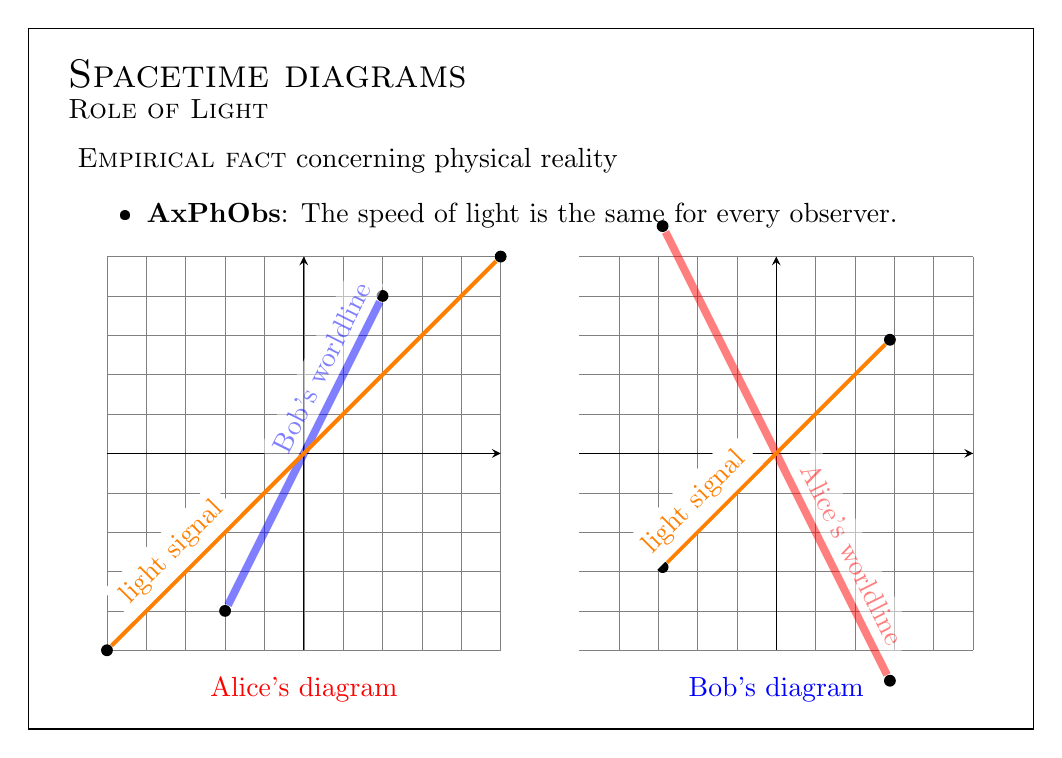
\begin{tikzpicture}[>=stealth, scale=1,
world/.style={inner sep=0, minimum size=.15cm, fill=black, circle},
worldline/.style={line width=1mm, rounded corners=1pt, opacity=.5},
axis/.style={->},
light/.style={orange, line width=.5mm},
]
\pgfmathdeclarefunction{XLorentz}{3}{\pgfmathparse{(#2 - #1*#3)/(sqrt(1-#1^2))}} % speed, spacecoord, timecoord
\pgfmathdeclarefunction{YLorentz}{3}{\pgfmathparse{(#3 - #1*#2)/(sqrt(1-#1^2))}} % speed, spacecoord, timecoord

%%%%%%%%%%%%%%%%%%%%%%%% DIA KEZDETE %%%%%%%%%%%%%%%%%%%%%%%%%%%

\node[anchor=north west, inner sep=0] at (0.5,8.5) {\textsc{\Large Spacetime diagrams}}; %%%%%%% TITLE
\node[anchor=north west, inner sep=0] at (0.5,8) {\textsc{\normalsize Role of Light}}; %%%%%%% SUBTITLE
\draw%[white]  %%%%%%%%%%%% SIZE OF THE SLIDE
      (0,0) rectangle (12.77,8.9);
%%%%%%%%% TEXT %%%%%%%%%%%%%
\node[anchor=north west] at (0.5,7.5) {\begin{minipage}{12cm}
\textsc{Empirical fact} concerning physical reality
\begin{itemize}
\item \textbf{AxPhObs}: The speed of light is the same for every observer.
\end{itemize}
\end{minipage}
};
%%%%%%%%%%%%%%%%%%%%%%%% KOORDINÁTARENDSZEREK %%%%%%%%%%%%%%%%%%%%%%%%%%%
\coordinate(O1) at (3.5,3.5);
  \CoordSys{O1}{2.5}{2.5}
\coordinate(O2) at (9.5,3.5);
  \CoordSys{O2}{2.5}{2.5}

%%%%%%%%%%
%% SETTINGS %%
%%%%%%%%%%


\coordinate (SignalStart) at (1,1) {} {};
\coordinate (SignalBounced) at (6,6) {};
\coordinate (AliceStart) at (3.5,1) {};
\coordinate (AliceEnd) at (3.5,6) {};
\coordinate (BobStart) at (2.5,1.5) {} {} {}; % Fontos hogy átmenjen az Origón, különben rossz a lorentz transzformáció!!
\coordinate (BobEnd) at (4.5,5.5) {} {} {};

%%%%%%%%%%% Ezt lehetne macronak, speedszámítócuccnak
\path (BobStart); \pgfgetlastxy{\XCoord}{\YCoord}; % Extracting coordinates of the Origin
\pgfmathsetmacro{\XFirst}{\XCoord} % Saving X coordinate
\pgfmathsetmacro{\YFirst}{\YCoord} % Saving Y coordinate
\path (BobEnd); \pgfgetlastxy{\XCoord}{\YCoord}; % Extracting coordinates of the Point
\pgfmathsetmacro{\XSecond}{\XCoord} % Saving X coordinate
\pgfmathsetmacro{\YSecond}{\YCoord} % Saving Y coordinate
\pgfmathsetmacro{\SpeedBob}{(\XFirst-\XSecond)/(\YFirst-\YSecond)} % Relativizing to the origin
%%%%%%%%%%%%%%%%%%%%%%%%%%%%%%%%%%%

\Lorentz{O1}{O1}{0}{BobStart}{BS}
\Lorentz{O1}{O1}{0}{BobEnd}{BE}
\Lorentz{O1}{O1}{0}{SignalStart}{SS}
\Lorentz{O1}{O1}{0}{SignalBounced}{SB}
\Lorentz{O1}{O2}{\SpeedBob}{AliceStart}{AS'}
\Lorentz{O1}{O2}{\SpeedBob}{AliceEnd}{AE'}
\Lorentz{O1}{O2}{\SpeedBob}{SignalStart}{SS'}
\Lorentz{O1}{O2}{\SpeedBob}{SignalBounced}{SB'}
\node[rotate=0, text=red, fill=white] at (3.5,0.5) {Alice's diagram};
\node[rotate=0, text=blue, fill=white] at (9.5,0.5) {Bob's diagram};
\draw[worldline, blue] (BS)--(BE) node[fill=white, sloped, above, pos=.75]{Bob's worldline};
\draw[worldline, red] (AS')--(AE') node[fill=white, sloped, above, pos=.25]{Alice's worldline};
\draw[light]  (SS)-- (SB) node[fill=white, sloped, above, pos=.2]{light signal};
\draw[light]  (SS')-- (SB') node[fill=white, sloped, above, pos=.2]{light signal};
\end{tikzpicture}